\documentclass[letterpaper]{article}

\usepackage{graphicx}
\usepackage{hyperref}
\usepackage{listings}
\usepackage{placeins}
\usepackage{float}
\usepackage[margin=1in]{geometry}

\begin{document}

% Title -----------------------------------------------------------------------

\title{CSE 40166 Final Report}
\date{12/15/17}
\author{Kyle Miller\\ {\textless}kmille42@nd.edu{\textgreater} \and Andrew Callahan\\ {\textless}acallah1@nd.edu{\textgreater} \and Christopher Clarizio\\ {\textless}cclarizi@nd.edu{\textgreater}}

\maketitle

% Overview --------------------------------------------------------------------

\section*{1. Overview}

\paragraph{}
	The original idea of our project was to create an animated simulation of a campfire. We planned to be able to choose to start and stop the fire using a button so that the simulation would show the fire would growing to its max size and then dissipating. We also planned that the fire would be textured, generate light and that the light generated by the fire would determine the lighting of the environment. Lastly, we planned to be able to move the camera around the scene using standard trackball controls.
\paragraph{}
    In order to implement our simulation we planned on using generally the same techniques that we implemented our homework assignments with. Specifically, we intended to use custom shaders and javascript code to create our simulation in the same way that we did for assignments such as the orrery. Additionally, in order to make the simulation more realistic, we intended to implement a function that would distort the flame using a system of splines and a function that would model the randomness of particles within the fire. Furthermore, we speculated that we would be able to simulate the effects of a breeze on the fire using another function that would again transform the shape of the fire.
\paragraph{}    
    In regards to our final iteration of our project, the idea is the same (a campfire simulation) and all but one of the planned features was implemented (growth/dissipation of fire was not implemented). However, we employed a significantly different method of implementation. Instead of using WebGL and creating custom shaders for our project we used THREE.js and a library for particle simulation after its usefulness was demonstrated in class.
    

% Main Functions --------------------------------------------------------------
\section*{2. Main Functions}

\paragraph{}
    Our project was implemented almost entirely in one file, "campfire.html". Within "campfire.html", it is split into a head and a body. The head is relatively unimportant as it only sets some of the styling used. The body is where all of our simulation is done. In the body we import the external scripts that we use later in our script including "three.js", "OrbitConrtorls.js", and "GPUParticleSysem.js". Then we define our script which does the main graphical work. Our script is split into three part. First, it sets up the options menu then the function "init" which sets the simulation up and finally the function "animate" which handles the animation. 
\paragraph{}    
    In regards to setting up the options menu, the first thing that we do is declare and initialize the variables that we will be able to control using the options menu such as "vel\_rand", "turbulence" and "lifetime". We then initialize "valController" to contain the variables that we will be able to control using the options menu. We then define our two event handler functions "valChanger" which handles changing the values of the attributes in "valController" when the options menu is used and "restartSimulation" which handles reseting the values of the variables in "valController" when the reset button in the options menu is pressed. Finally, we add our variables to the options menu using "gui.add" and add the proper event handler funcition to them using ".onchange" to link each option to either "valController" or "restartSimulation".
\paragraph{}    
    Our function "init", as its name suggests, sets up our simulation. First, we get a reference to the area that we want to draw in using "document.getElementById" and stores it into "container". Then we set up the camera using "THREE.PerspectiveCamera" to initialize it and "camera.x", "camera.y", and "camera.z" to set its position. Then we initialize our scene using "THREE.scene". Then we add the geometries for the ground and moon using "THREE.SphereBufferGeometry" and "THREE.PlaneBufferGeometry" respectively. For the ground we first create a mesh using "THREE.MeshPhongMaterial". We then load in our textures for the ground using "textureLoader.load" three times for the texture, bump map and roughness map. We use the same technique to create meshes and load textures for the moon and the rocks in our simulation but we only call "textureLoader.load" once for each since we only load a texture and not a bump map or roughness map. We then use a for loop to combine the geometry from the moon (a generic sphere) and the texture we just loaded for the rocks to add the rocks to our simulation using "THREE.mesh" and "scene.add". Then we do the same thing for the moon and ground again using "THREE.mesh" and "scene.add". After that we add three lights to the scene: a point light to simulate the fire's light, and a directional and point light to simulate the moon's light. We do this using "THREE.PointLight" and "THREE.DirectionalLight" to create the lights, ".position.set" to set their positions and "scene.add" to add them to the scene. Additionally, for the directional light we set the direction using "moonlight.target = sphere" to point it towards the the sphere that is used for the moon. Then we add the logs to our simulation using the same techniques used for the rocks and the moon, however we use "THREE.CylinderGeometry" to get the proper shape. In order to set up the particle systems that simualte the flame we iterate to initialize and add "nSystems" number of particle systems to the scene using "THREE.GPUParticleSystem" and "scene.add" and we set the "options" and "spawnerOptions" to their default values. Then we add the sound to the simulation by making a listener using "THREE.AudioListener", adding the listener to the camera and loading the sound using "audioLoader.load". Finally, we set the options of the renderer, set the options of the controls and add an event listener for window resizing. 
\paragraph{}
    Our function "animate" handles animating our simulation. Within our "animate" we specify that "animate" is our animation function using "requestAnimationFrame". We then calculate the time that has passed since the last frame by setting "delta" to the result of "clock.getDelta" scaled by "spawnerOptions.timescale". We then incriment "tick" by "delta" and if "delta" is greater than zero (i.e. if some time has passed since the last frame) we set the options for the point light in the flame to a semi-random value to model the flickering of the flame and set the position of the particle systems to be along the outline of a tear drop shape. Finally, we iterate through the particle systems in our simulation and call their update functions and then the render function to render to the scene. 

% How to Use the Program ------------------------------------------------------
\section*{3. How to Use}

\paragraph{}
    Our project is extremely simple to use. Once you load the page the simulation will begin and you will see the campfire and the accompanying scene (i.e. logs, stones, ground and moon). You can rotate the camera by using standard trackball controls and zoom the camera in and out by using the scrollwheel on your mouse. The trackball controls, however, will not allow you to rotate beyond certain angles (i.e. it will not allow you to rotate the camera so that is below the ground). You can also adjust certain attributes of the fire such as color and size using sliders that are in a dropdown menu in the upper-right-hand corner. Lastly, you can reset and restart the simulation by clicking the button at the bottom of the dropdown menu.

% Program Results-------- ------------------------------------------------------
\section*{4. Results}

\begin{figure}[H]
\centering
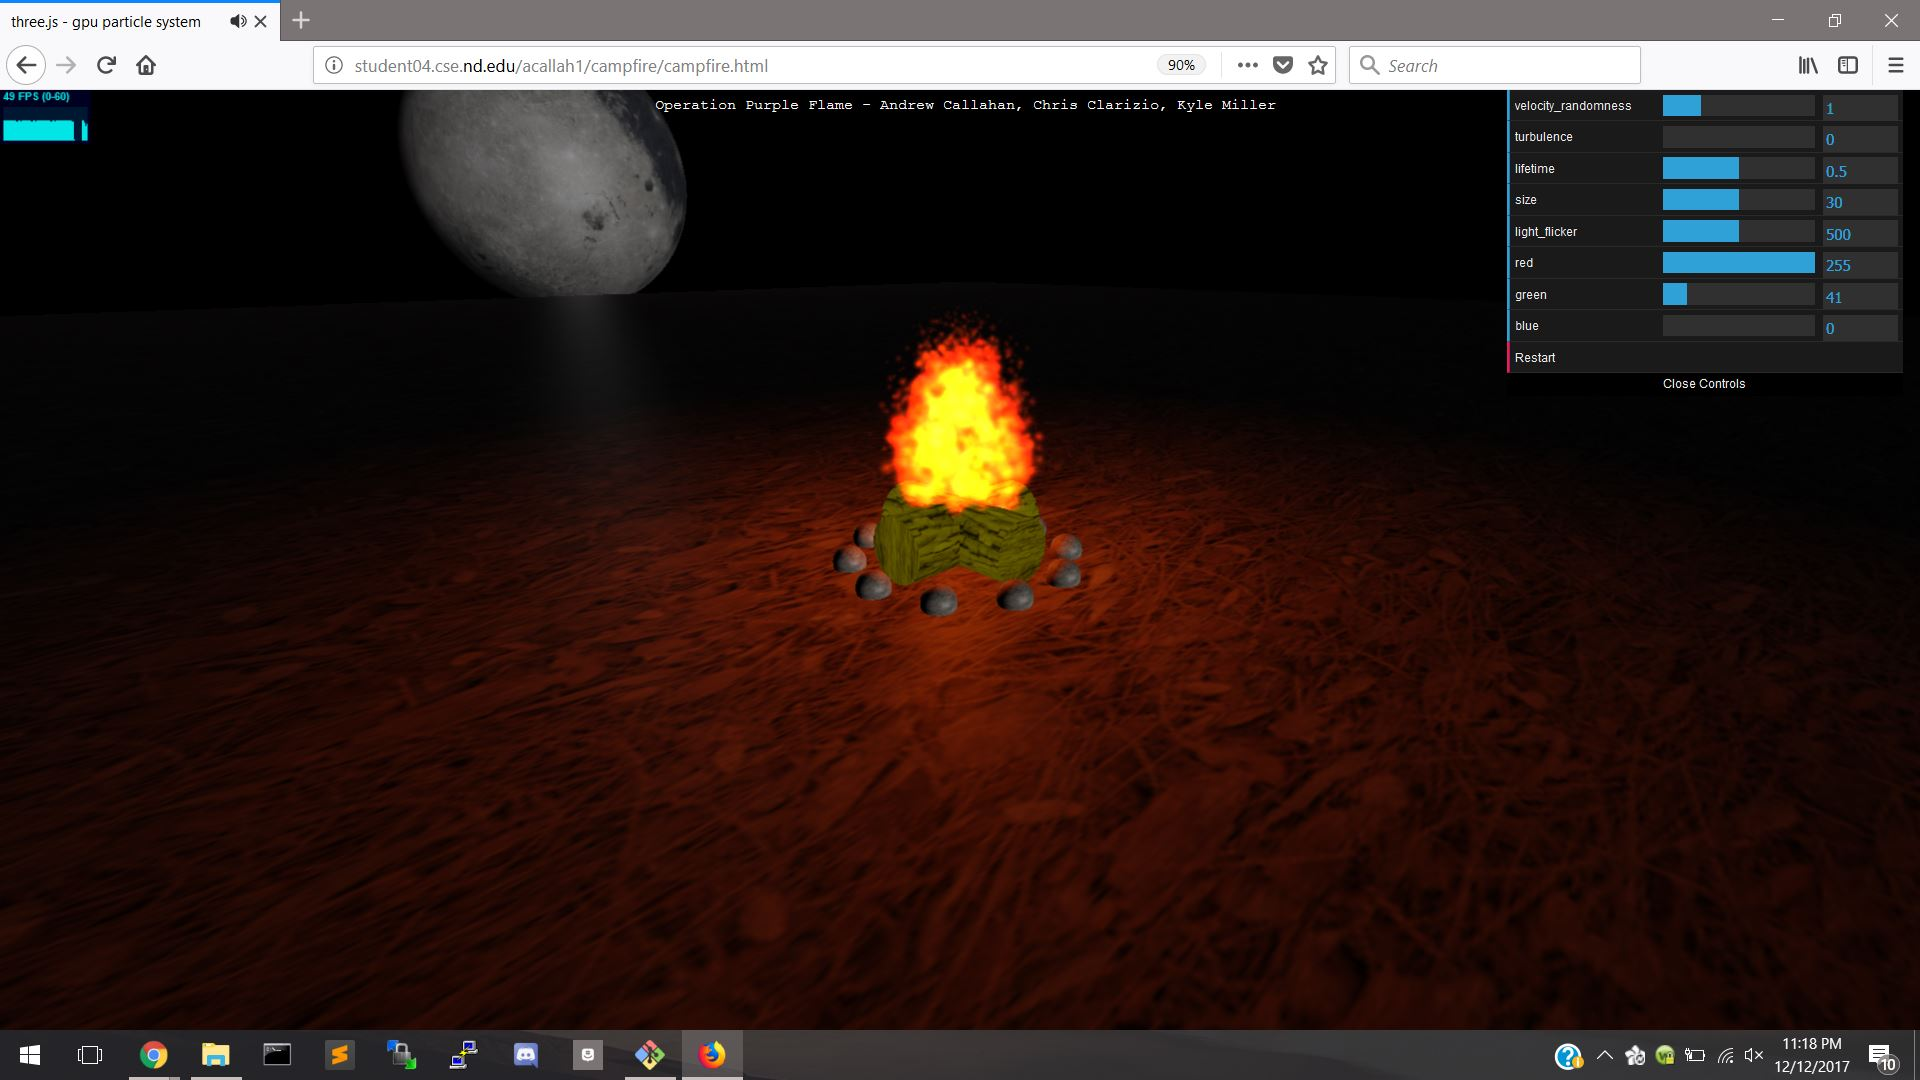
\includegraphics[scale=.35]{result1.JPG}
\caption{Basic Campfire}
\label{fig:result1}
\end{figure}
\paragraph{}
This is a still image of our simulation with its default settings. It shows the point light inside the fire casting light on the ground, the moon being lit by its point and directional light, and the randomness of the particles that simulate the flame.

\begin{figure}[H]
\centering
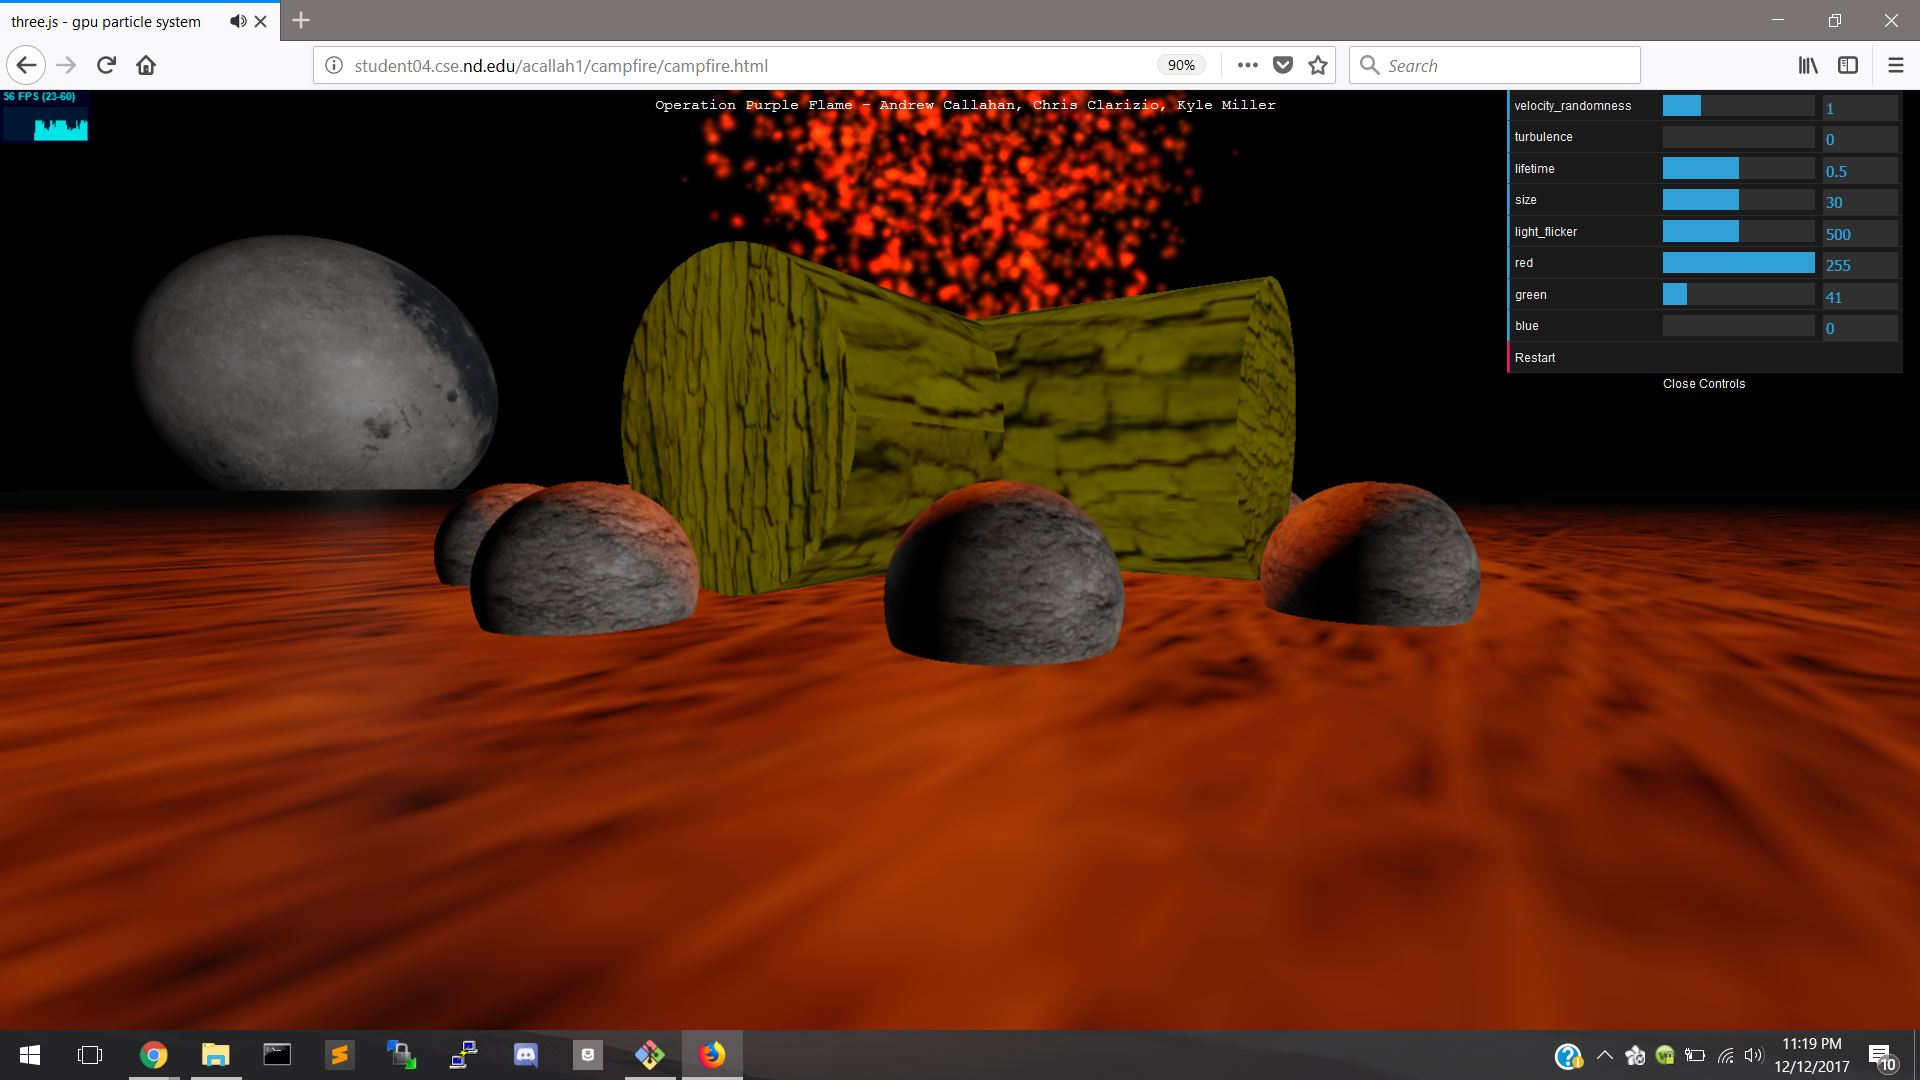
\includegraphics[scale=.35]{result2.JPG}
\caption{Moon, Rocks, Stones}
\label{fig:result2}
\end{figure}
\paragraph{}
This illustrates the ability to move the camera, that the logs are cylinders with the same texture and that the rocks are spheres with the same texture.

\begin{figure}[H]
\centering
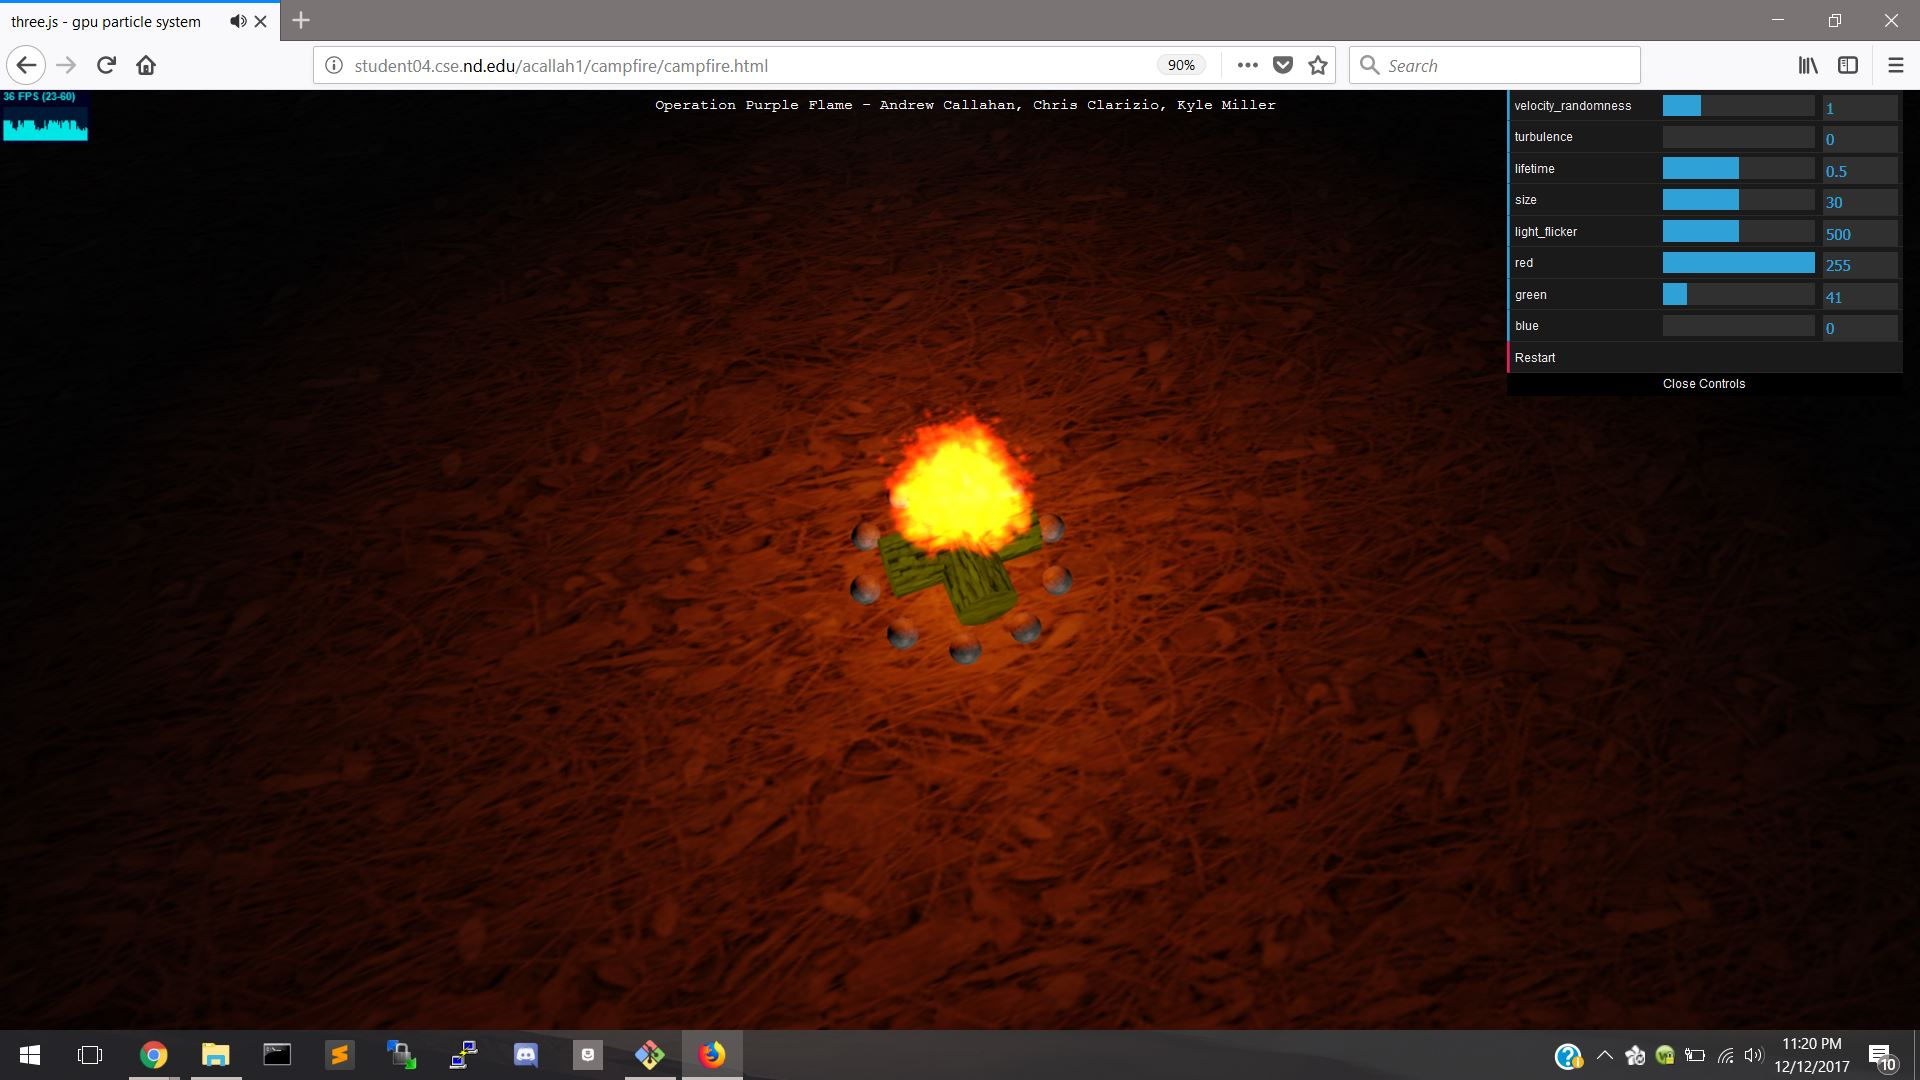
\includegraphics[scale=.35]{result3.JPG}
\caption{Overhead View}
\label{fig:result3}
\end{figure}
\paragraph{}
This illustrates again the ability to move the camera and that the ground is textured and has a bump map.

\begin{figure}[H]
\centering
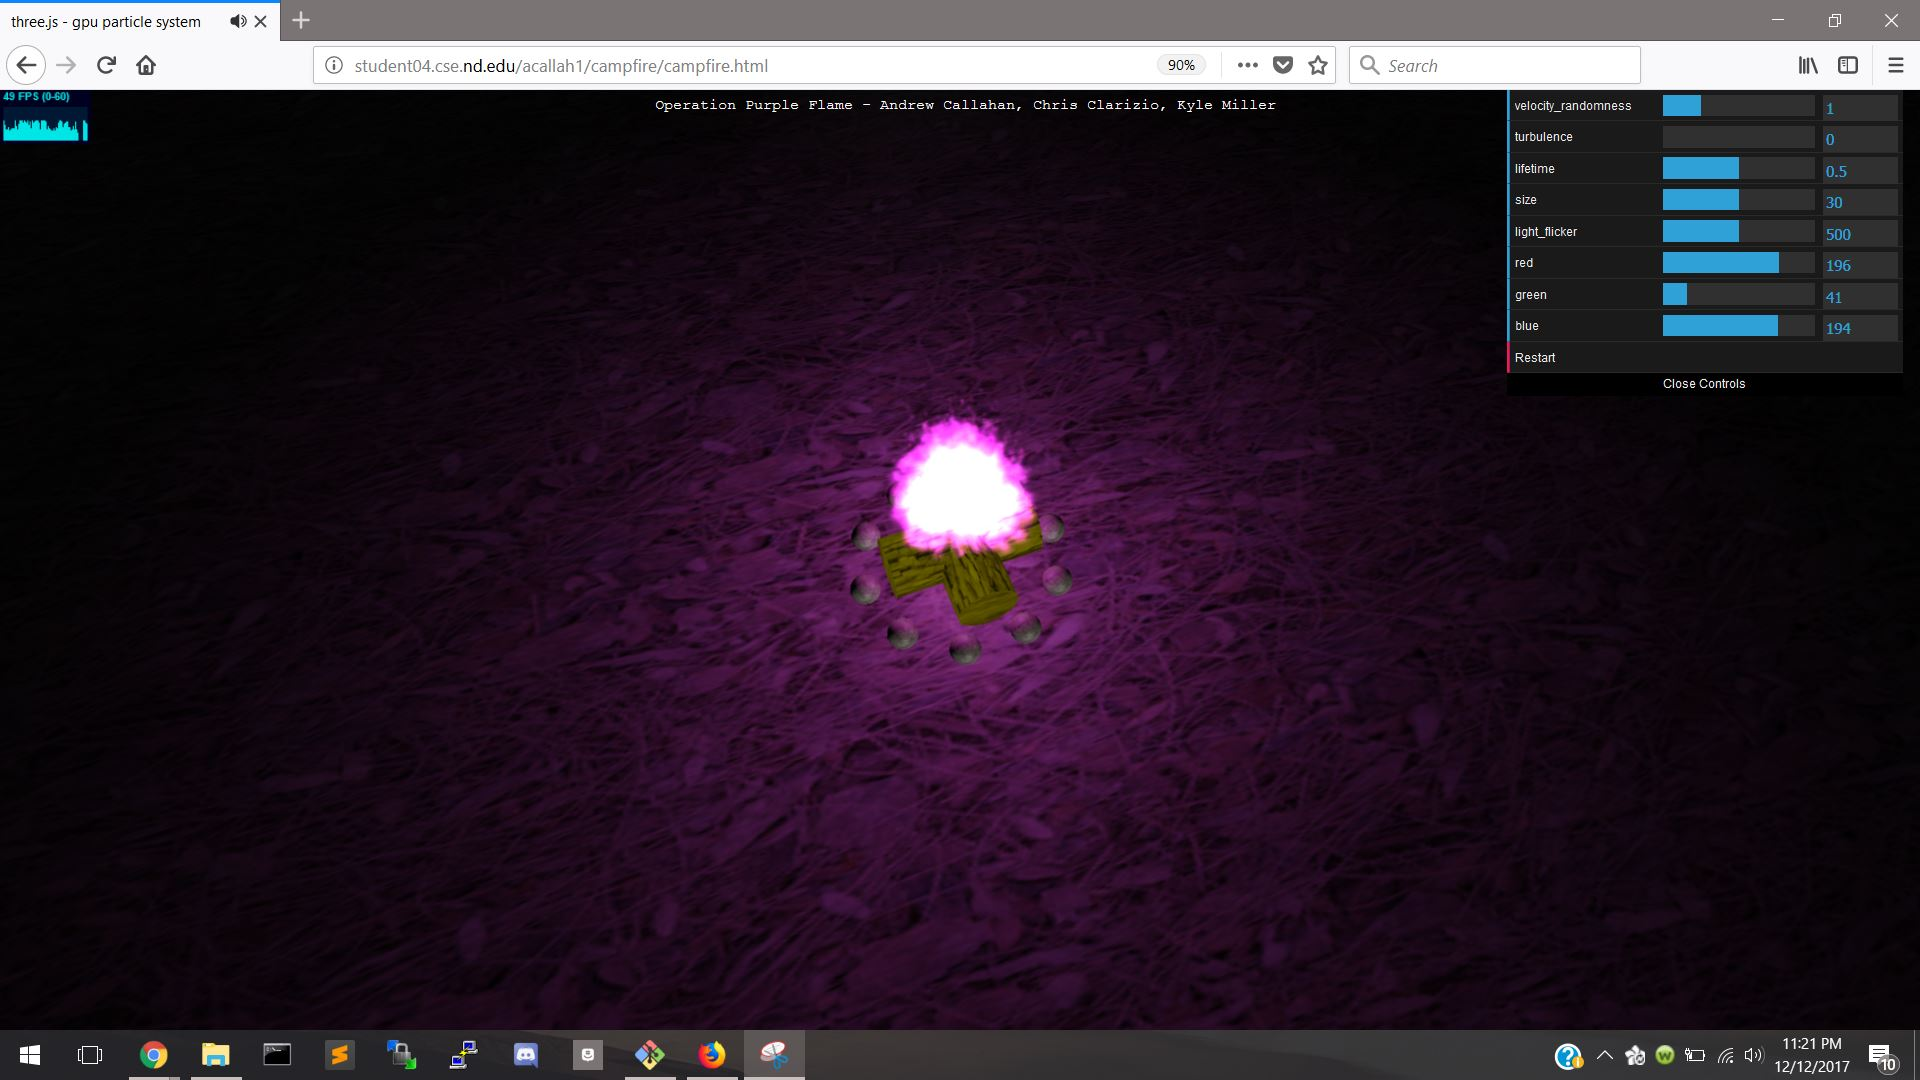
\includegraphics[scale=.35]{result4.JPG}
\caption{Colored Campfire}
\label{fig:result4}
\end{figure}
\paragraph{}
This illustrates the ability to change the color of the flame using the r,g,b sliders in the options menu.

\begin{figure}[H]
\centering
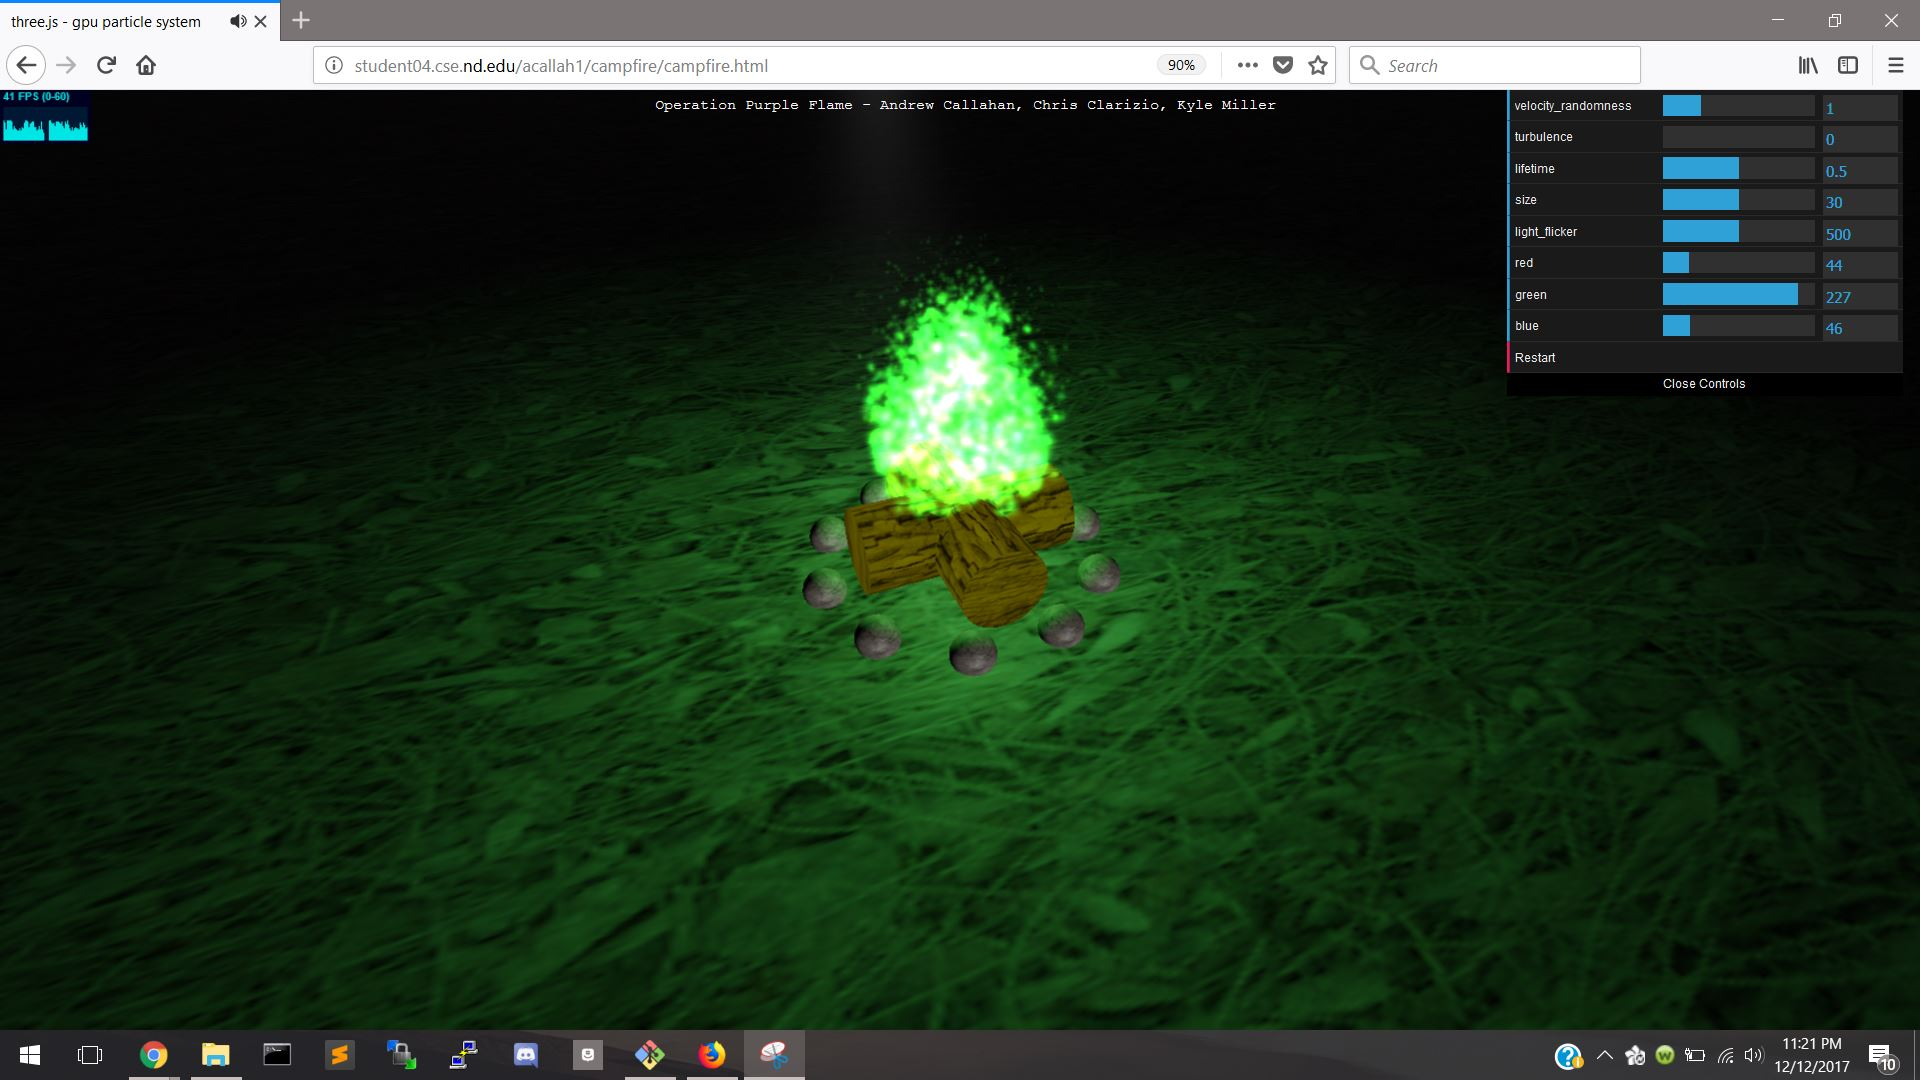
\includegraphics[scale=.35]{result5.JPG}
\caption{Colored Campfire}
\label{fig:result5}
\end{figure}
\paragraph{}
This again illustrates the ability to change the color of the flame using the r,g,b sliders in the options menu.

\begin{figure}[H]
\centering
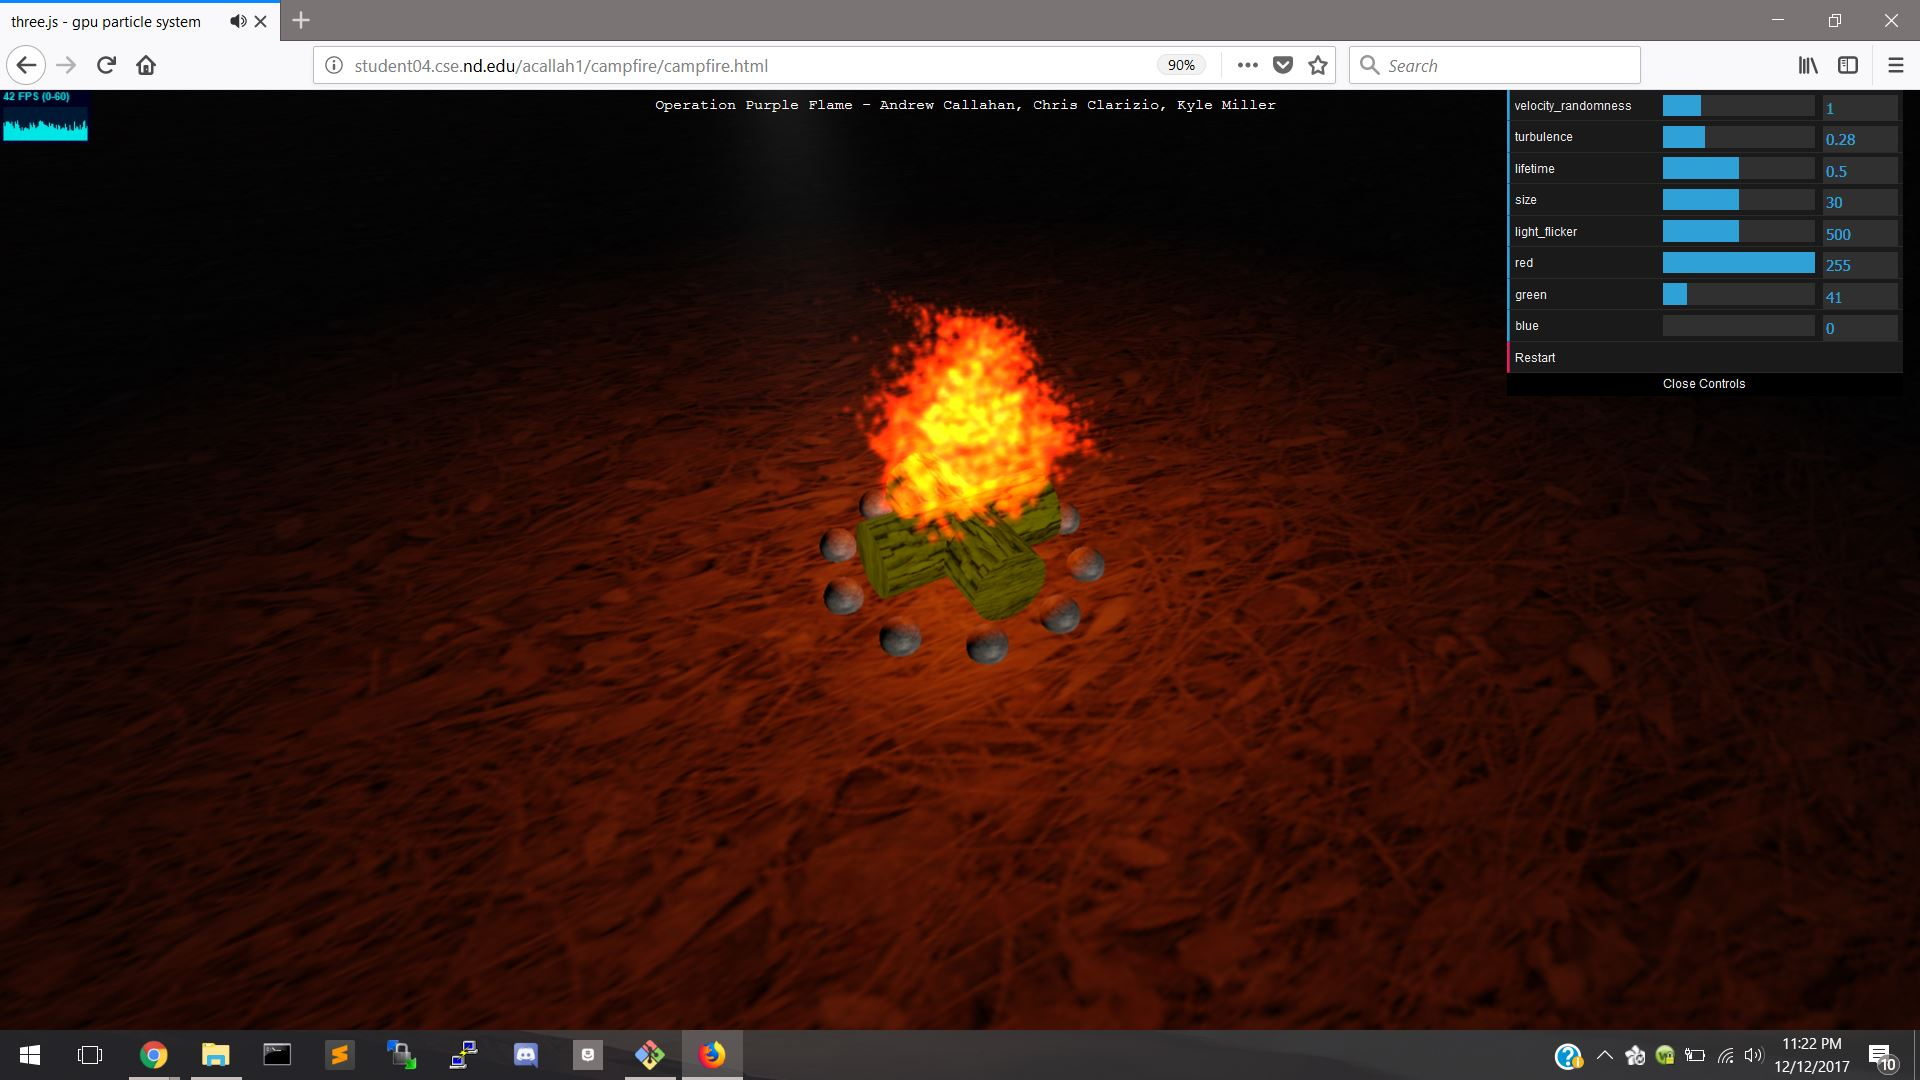
\includegraphics[scale=.35]{result6.JPG}
\caption{Turbulent Campfire}
\label{fig:result6}
\end{figure}
\paragraph{}
This illustrates the ability to change how turbulent the particles are and thus affect the flame's simulation.

\begin{figure}[H]
\centering
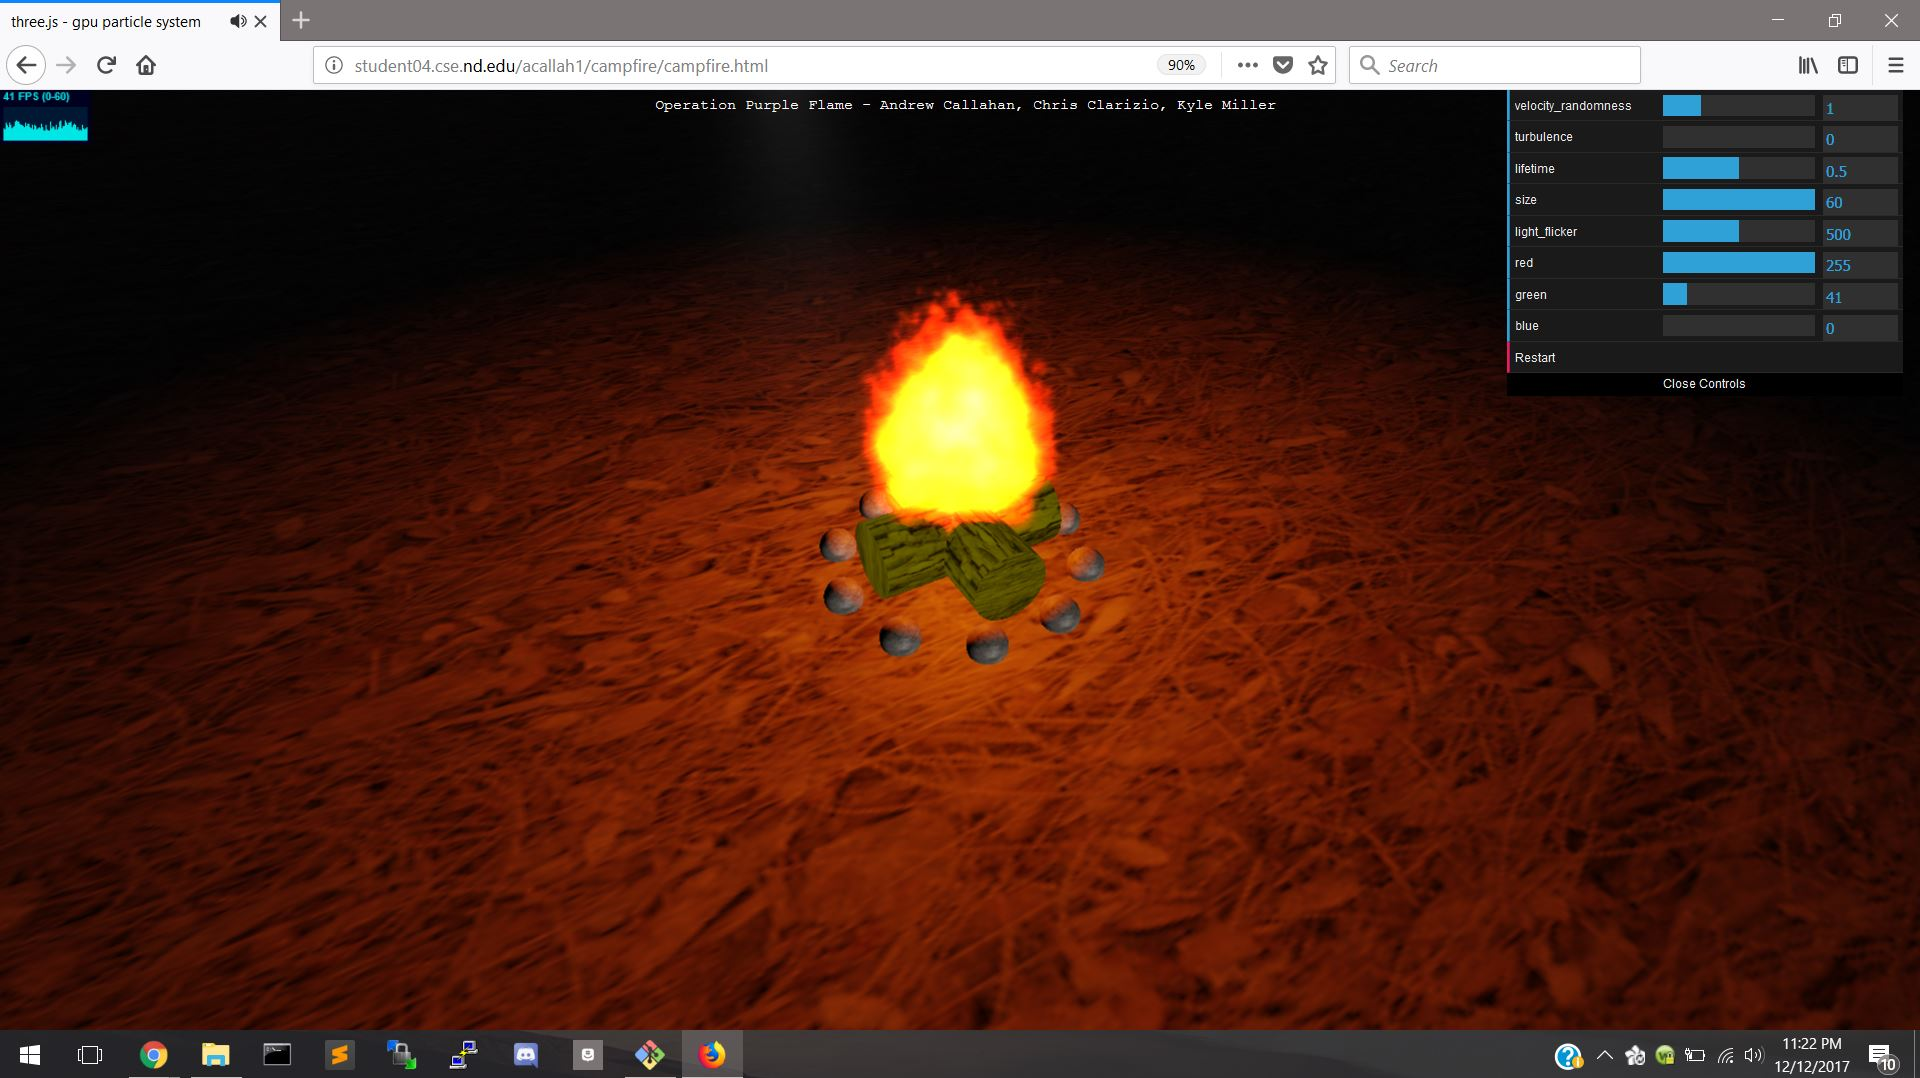
\includegraphics[scale=.35]{result7.JPG}
\caption{Campfire with Large Size}
\label{fig:result7}
\end{figure}
\paragraph{}
This illustrates the ability to change the size of the particles and thus affect the simulation of the flame by making it to appear smoother.

\begin{figure}[H]
\centering
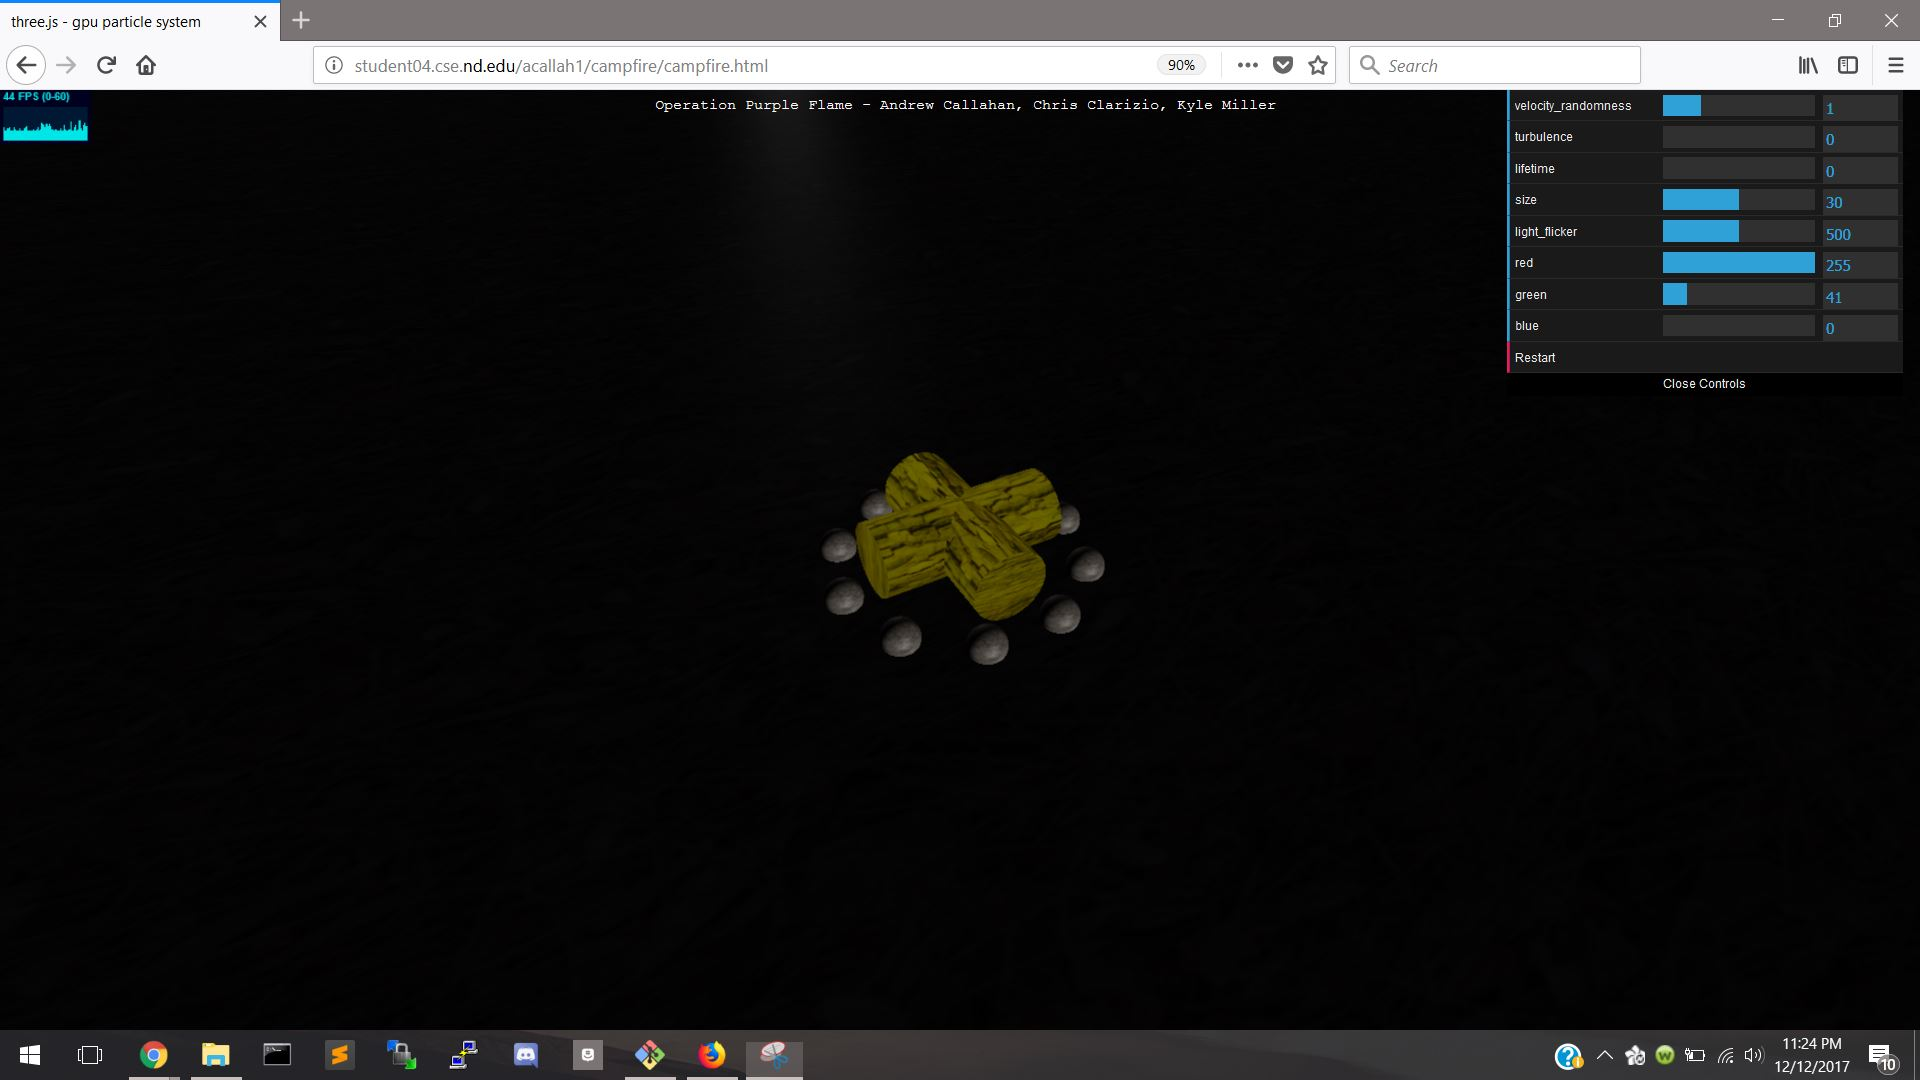
\includegraphics[scale=.35]{result8.JPG}
\caption{Campfire with Lifetime Zero}
\label{fig:result8}
\end{figure}
\paragraph{}
This illustrates the ability to change the lifetime of the particles (even to zero) and affect whether the flame is visible at all.

\begin{figure}[H]
\centering
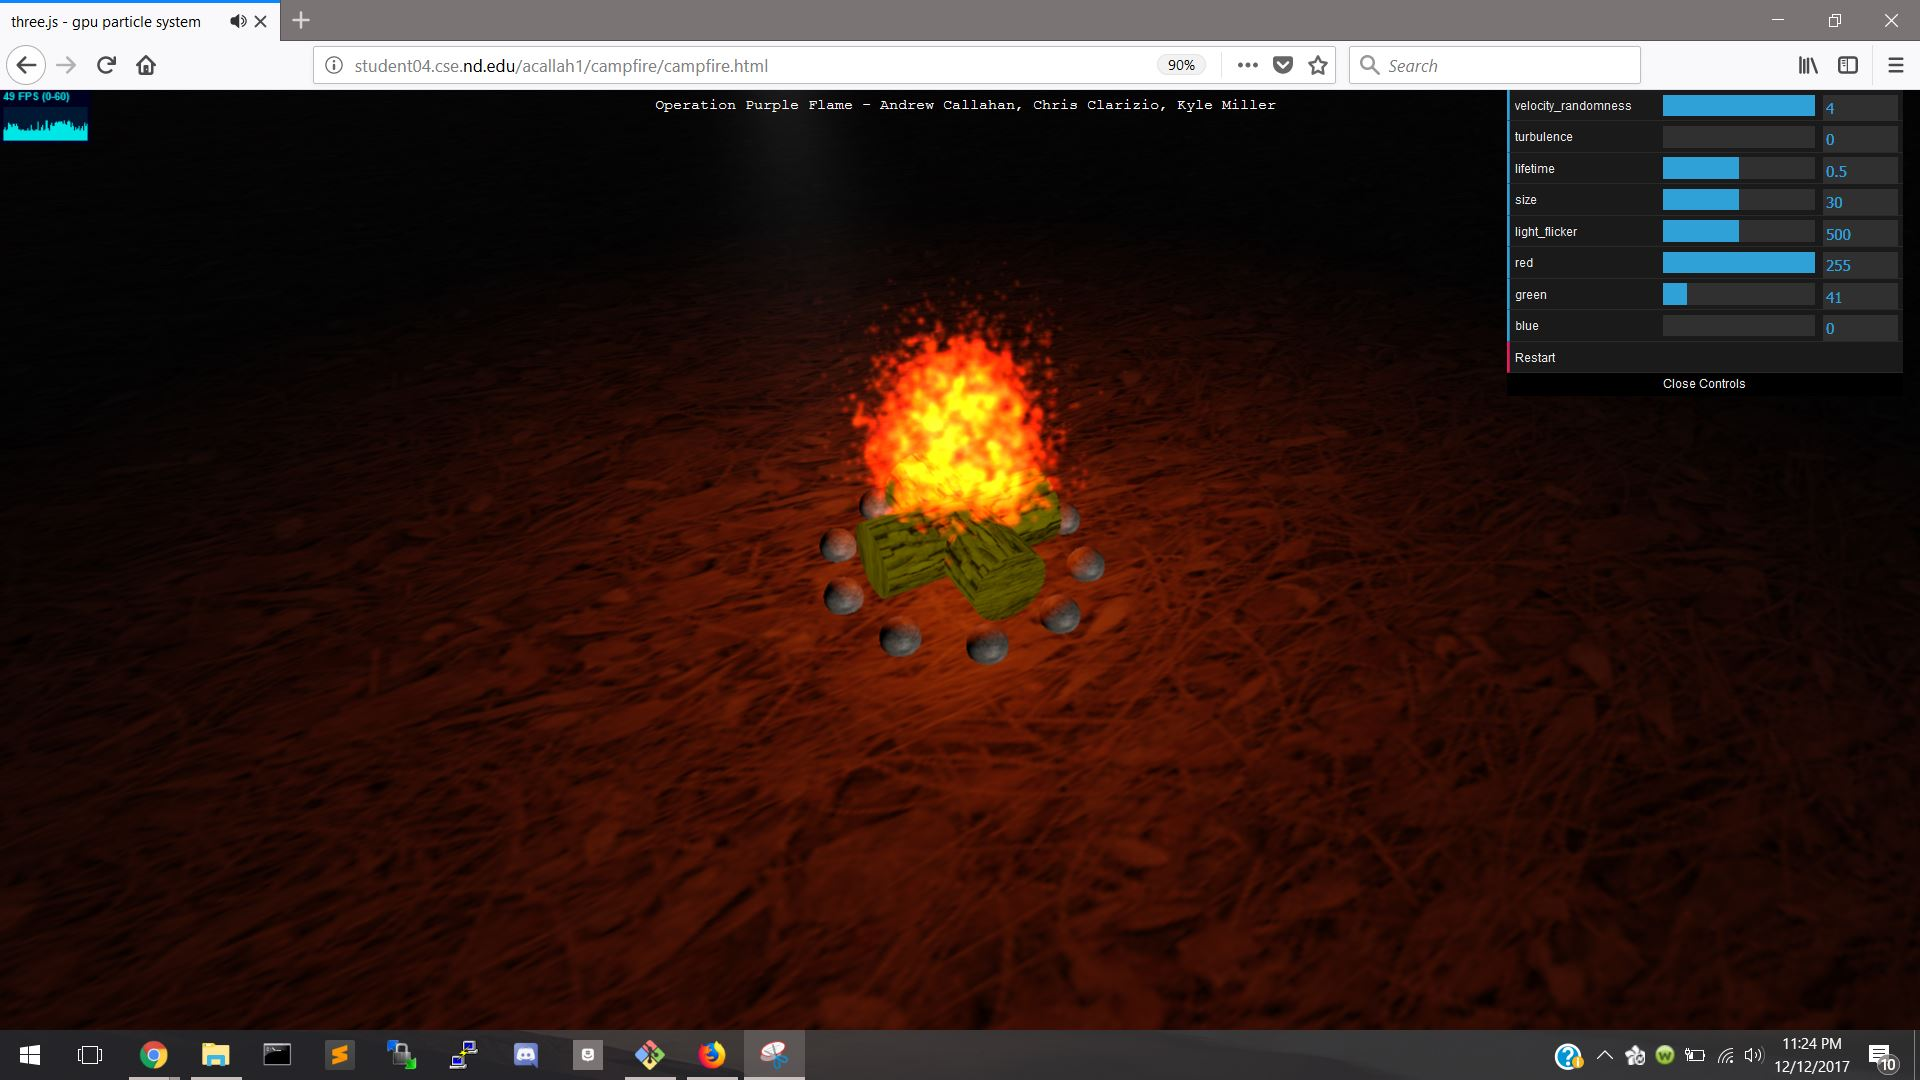
\includegraphics[scale=.35]{result9.JPG}
\caption{Campfire with Highly Random Velocities}
\label{fig:result9}
\end{figure}
\paragraph{}
This illustrates the ability to change how random the particles' velocities are and thus affect the simulation of the flame by making it appear to spread more and be more scattered.


% Technical Challenges -------------------------------------------------------
\section*{5. Technical Challenges}

\paragraph*{}
    filler text

% Assessement of Other Team Members ------------------------------------------
\section*{6. Assessment of Other Team Members}

\paragraph*{}
    filler text
% What I Learned -------------------------------------------------------------
\section*{7. What Was Learned}

\paragraph*{}
    filler text

\end{document}
